\documentclass[12pt,a4paper]{report}
\usepackage[utf8]{inputenc}
\usepackage[french]{babel}
\usepackage[T1]{fontenc}
\usepackage{amsmath}
\usepackage{amsfonts}
\usepackage{tcolorbox}
\newtcolorbox{mybox}[1]{colback=blue!5!white,colframe=blue!60!black,fonttitle=\bfseries,title=#1}

\newtcolorbox{Cas1}[1]{colback=green!5!white,colframe=green!60!black,fonttitle=\bfseries,title=#1}

\newtcolorbox{Cas2}[1]{colback=yellow!5!white,colframe=yellow!60!black,fonttitle=\bfseries,title=#1}


\newtcolorbox{Cadre}{colback=red!5!white,colframe=red!75!black}

\usepackage[Sonny]{fncychap}
\usepackage{listings}
\usepackage{amssymb}
\usepackage{graphicx}
\usepackage[left=2cm,right=2cm,top=2cm,bottom=2cm]{geometry}
\author{ADOLPHE Benjamin-BERJOLA Matthias}
\title{Multiplication Russe}
\begin{document}


\title{Multiplication Russe}
\author{ADOLPHE Benjamin-BERJOLA Matthias}


\maketitle 

\newpage
\chapter{Introduction}
\begin{large}
\begin{flushleft}
Dans le cadre de l'UE calculabilité et complexité nous avons dû réaliser plusieurs tâches sur un algorithme comprenant un contrat pré-conditions/post-conditions clair, et incluant au moins une boucle tant-que.Nous avons choisis de travailler sur l'algorithme représentant la multiplication russe et d'effectuer les tâches suivantes sur ce dernier: 

\begin{itemize}
\item[•] Écrire son code Dafny
\medskip

\item[•] Montrer la correction totale:
\begin{itemize}
\item[•] Montrer la  correction partielle : les invariants seront présentées et prouvés, ainsi que les post-conditions.
\medskip

\item[•] Prouver sa terminaison : fonctions de rang et éventuels invariants seront présentées et prouvés
\medskip 
\end{itemize}

\item[•] Déterminer sa complexité en temps qui dans le pire des cas sera justifiée et possiblement validée expérimentalement

\medskip

Nous allons donc exposé nos travaux dans ce rapport en prenant soin de suivre l'ordre décrit ci-dessus
\end{itemize}
\end{flushleft}
\end{large}

%*********************************
%*******Code Dafny**************											   
%*********************************                                                
%*********************************
\chapter{Code en Dafny}
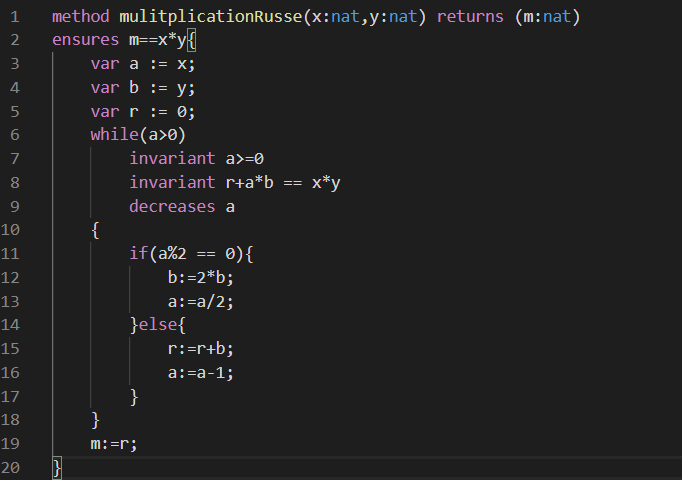
\includegraphics[scale=0.45]{algoDafny} 
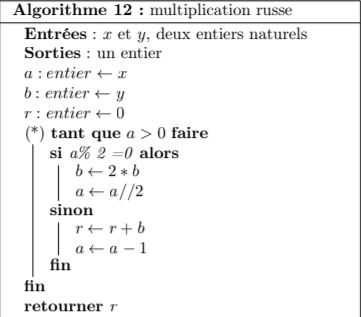
\includegraphics[scale=0.5]{algoRusse} 



%*********************************
%*******Correction totale******											   
%*********************************                                                
%*********************************

\chapter{Correction totale}
\section{Correction partielle}
\begin{mybox}{Méthode de détermination de la correction partielle}
On commence par déterminer l'invariant de boucle en posant les cas de base
et de récursivité.
\end{mybox}
\begin{flushleft}
Invariant en (*) $  a\geq 0 $  : \\
\begin{itemize}
\item Cas Inductif :  $x$ est affect\'{e} \`{a} $a$ or $x$ est un entier naturel ainsi par typage $a\ge 0$.
\item Cas Récursif : nous supposons que l'invariant  $a\ge 0$ est vrai, montrons alors $ a' \geq 0 $ :
\begin{itemize}
\item[•]  1\up{er} cas :  est pair. Nous savons que $\left[ \begin{array}{c}(a\ge 0\wedge a>0\wedge \\
   a '=(\frac{a}{2})\wedge a\%2=0 \wedge \\
b '=2*b\wedge r '=r)\end{array}
\right]$. Ainsi nous avons $a\ge 0\Leftrightarrow \frac{a}{2}\ge \frac{0}{2}\Leftrightarrow a ' \ge 0$.
\item[•] 2\up{ème} cas : a est impair. Nous savons que $\left[ \begin{array}{c}(a\ge 0\wedge a>0\wedge \\
   r '= r+b\wedge b'=b  \wedge \\
a '=a+1\wedge a\%2=1\end{array}
\right]$. Ainsi nous avons  $a\ge 0$ d’après le test de boucle or  $  a\geq 0  \Leftrightarrow a-1 \ge 0-1 \Leftrightarrow a' \ge 0$ .
\bigskip
\end{itemize}
\end{itemize}
\begin{Cas1}{Conslusion}
 Dans les deux cas, nous avons bien montré que  $ a' \ge 0 $. $a \geq 0$ est donc bien un invariant de boucle en $(*)$ .
\end{Cas1}
\end{flushleft}

\begin{flushleft}
Invariant $(*) r+a*b = x*y$ :
\begin{itemize}
\item Cas Inductif : 0   est affecté à r, x  est affecté à a  et y   est affecté à b  ainsi $ r +a*b = 0 + a*b = x*y $. On a donc bien $ r + a*b = x*y$ .
\item Cas Récursif : nous supposons que l'invariant  $ r + a*b = x*y$ est vrai, montrons alors que  $ r' + a'*b' = x'*y'$ est vrai :
\begin{itemize}
\item[•]  1\up{er} cas : a est pair.  Nous savons que $\left[ \begin{array}{c}(r + a*b = x*y\wedge a>0\wedge \\
a\%2=0\wedge a'= \frac{a}{2} \wedge r'=r \wedge\\
b'=2*b\wedge x'=x \wedge y'=y\end{array}
\right]$.  Ainsi nous avons $ r' + a'*b' = r' + \frac{a}{2} * 2 * b  = r+ a*b$ or d’après
 invariant $ r+a*b = x*y $ et  $ x*y = x'*y'$. Nous avons donc bien $ r'+a'*b' = x'*y'$.
\item[•] 2\up{ème} cas : a est impair. Nous savons que $\left[ \begin{array}{c}(r + a*b = x*y\wedge a>0\wedge \\
a\%2=1\wedge a'= a-1\wedge b'=b \wedge\\
r'=r+b\wedge b'=b\wedge x'=x \wedge y'=y\end{array}
\right]$. Ainsi nous avons $r'+ a'*b'=r+b+(a-1)*b = r+a*b + b-b = r+a*b  $ or d’après l'invariant nous avons  $ r+a*b = x*y $et $ x*y = x'*y' $. Nous avons donc bien $ r'+a'*b' = x'*y'$.
\end{itemize}
\end{itemize}
\begin{Cas1}{Conclusion}
 Dans les deux cas, nous avons montré que $ r'+a'*b'= x'*y' $.
$ r+a*b=x*y $ est donc un invariant de boucle en $(*) $.
\end{Cas1}
\end{flushleft}

\section{Terminaison}
\begin{mybox}{Méthode de détermination de la terminaison}
On détermine une fonction de rang et on prouve que celle-ci est valide. C'est-à-dire, on vérifie que la fonction de rang $\in\mathbb{R}$ au point T1 et qu'elle décroit lorsque l'exécution passe entre les points T1 et T2.
\end{mybox}

\begin{flushleft}
Fonction de rang à valeur dans $\mathbb{N}$:
\begin{itemize}
\item \`A chaque passage au point T1, montrons que $a \in \mathbb{N}$. D'après l'invariant de boucle $a \ge 0$ nous savons donc que $a \in \mathbb{N}$.
\item \`A chaque fois que l'exécution passe entre le point T1 et le point T2, montrons que $a$ décroit strictement.
\begin{itemize}
\item[•] 1\up{er} cas: a est pair.Nous savons que $\left[ \begin{array}{c}(r + a*b = x*y\wedge a>0\wedge \\
a\%2=0\wedge a'= \frac{a}{2} \wedge r'=r \wedge\\
b'=2*b\wedge x'=x \wedge y'=y\end{array}
\right]$. Ainsi nous avons $a'=\frac{a}{2}$ donc $a>\frac{a}{2} \Leftrightarrow a>a'$. Nous avons bien $a$ strictement décroissante.
\item[•] 2\up{ème} cas: a est impair. Nous savons que $\left[ \begin{array}{c}(r + a*b = x*y\wedge a>0\wedge \\
a\%2=1\wedge a'= a-1\wedge b'=b \wedge\\
r'=r+b\wedge b'=b\wedge x'=x \wedge y'=y\end{array}
\right]$. Ainsi nous avons $a'=a-1$ donc $a>a-1 \Leftrightarrow a>a'$. Nous avons bien $a$ strictement décroissante.
\end{itemize}
\end{itemize}
\begin{Cas1}{Conclusion}
 Dans les deux cas, nous avons montré que $a$ est strictement décroissante. $a$ est donc une fonction de rang à valeur dans $\mathbb{N}$.
\end{Cas1}
\end{flushleft}
%*********************************
%*******Complexité**************											   
%*********************************                                                
%*********************************

\chapter{Complexité}

\end{document}
